\hsection{Installing Psycopg}%
\label{sec:installPsycopg}%
%
Since the installation of the programming language \python\ and the \pgls{ide} \pycharm\ is already covered in~\cite{programmingWithPython}, we will not reproduce this information here.
However, the installation of \psycopg\ is specific to this course, so we will discuss it in a bit more detail.

There are two ways to install this library:
If you execute a \db\ application written in \python\ in a productive environment, you will install \psycopg\ into a \pgls{virtualEnvironment} via the command line in a terminal.
Once this is done, you would activate the \pgls{virtualEnvironment} and be able to execute your application.
If you are either developing software locally or just want to explore the examples of this course, then you could install \psycopg\ within a \pgls{virtualEnvironment} under the \pycharm\ \pgls{ide}.
Both approaches to install packages have been covered in~\cite{programmingWithPython}.

Nevertheless, since they are integral to the contents of this course, we will also discuss them here.
It would best, however, if you would read~\cite{programmingWithPython} to a point where you know what \pip\ is and what \pglspl{virtualEnvironment} are.
We also cover the installation only under \ubuntu\ \linux, as the installation steps under \microsoftWindows\ will be analogous~(see again~\cite{programmingWithPython}).%
%
\hsection{Installing Psycopg via the Terminal}%
%
\begin{figure}%
\centering%
%
\subfloat[][%
We first open a \pgls{terminal} using \ubuntuTerminal.
We navigate to the directory where our programming will take place. %
We now create a directory \textil{.venv} to host a new \pgls{virtualEnvironment} by typing \bashil{mkdir .venv} and hitting~\keys{\enter}.%
\label{fig:pipInstallPyscopgVenv1mkdir}%
]{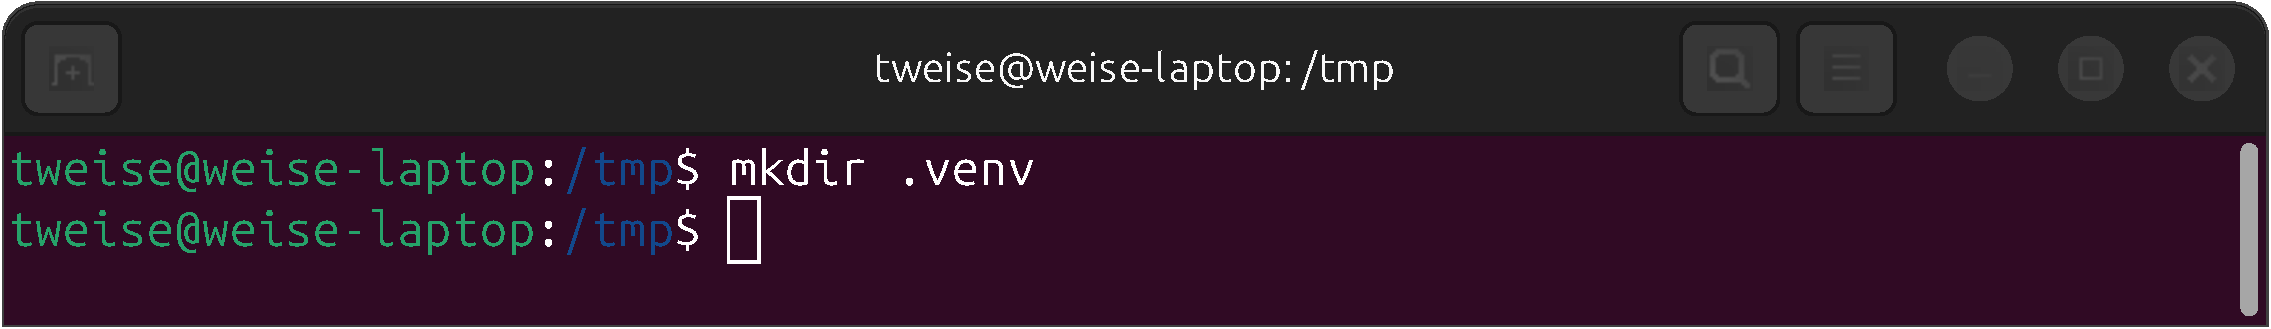
\includegraphics[width=0.7\linewidth]{\currentDir/pipInstallPyscopgVenv1mkdir}}%
%
\floatRowSep%
%
\subfloat[][%
We now set up a new and empty \pgls{virtualEnvironment} in this directory by writing \bashil{python3 -m venv --upgrade-deps .venv} and hitting~\keys{\enter}.%
\label{fig:pipInstallPyscopgVenv2venv}%
]{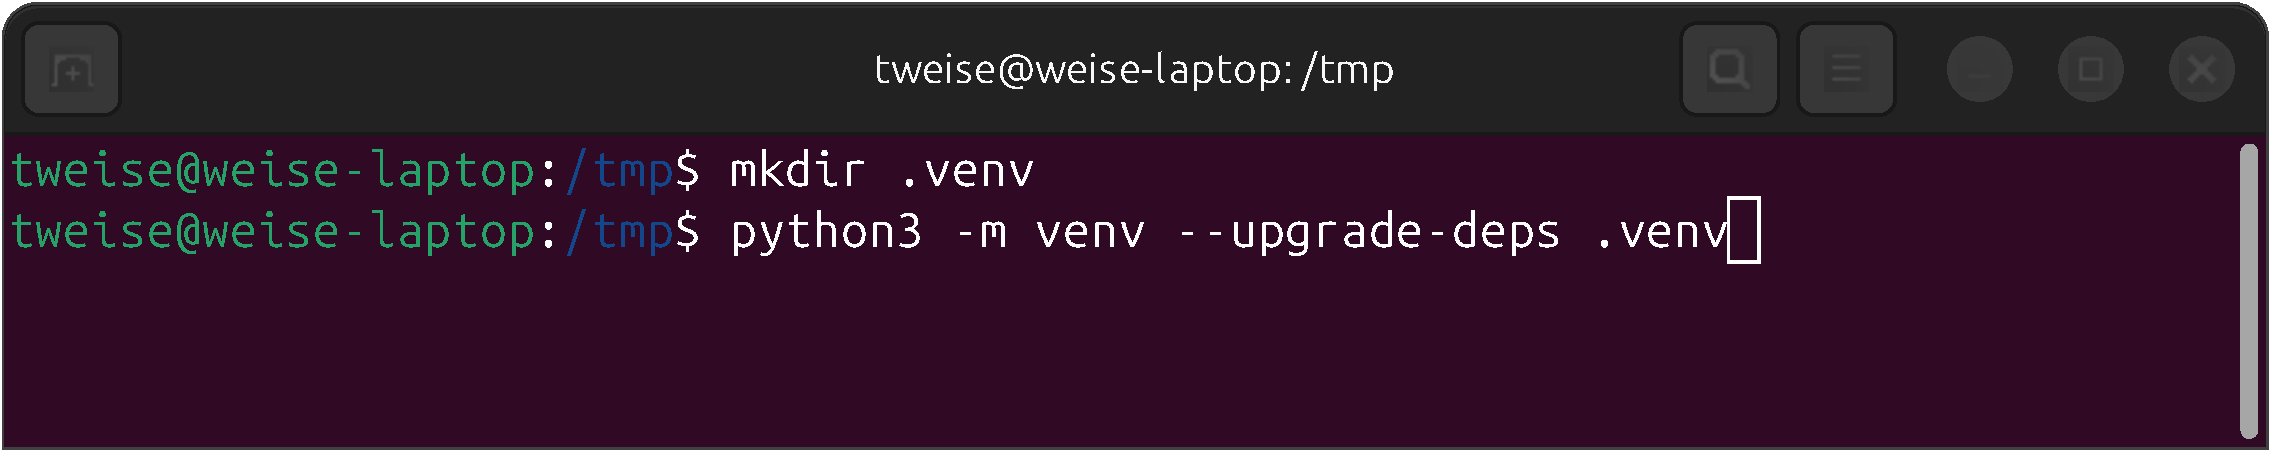
\includegraphics[width=0.7\linewidth]{\currentDir/pipInstallPyscopgVenv2venv}}%
%
\floatRowSep%
%
\subfloat[][%
The \pgls{virtualEnvironment} has been created. %
We now activate it by writing \bashil{source .venv/bin/activate} and hitting~\keys{\enter}.%
\label{fig:pipInstallPyscopgVenv3activate}%
]{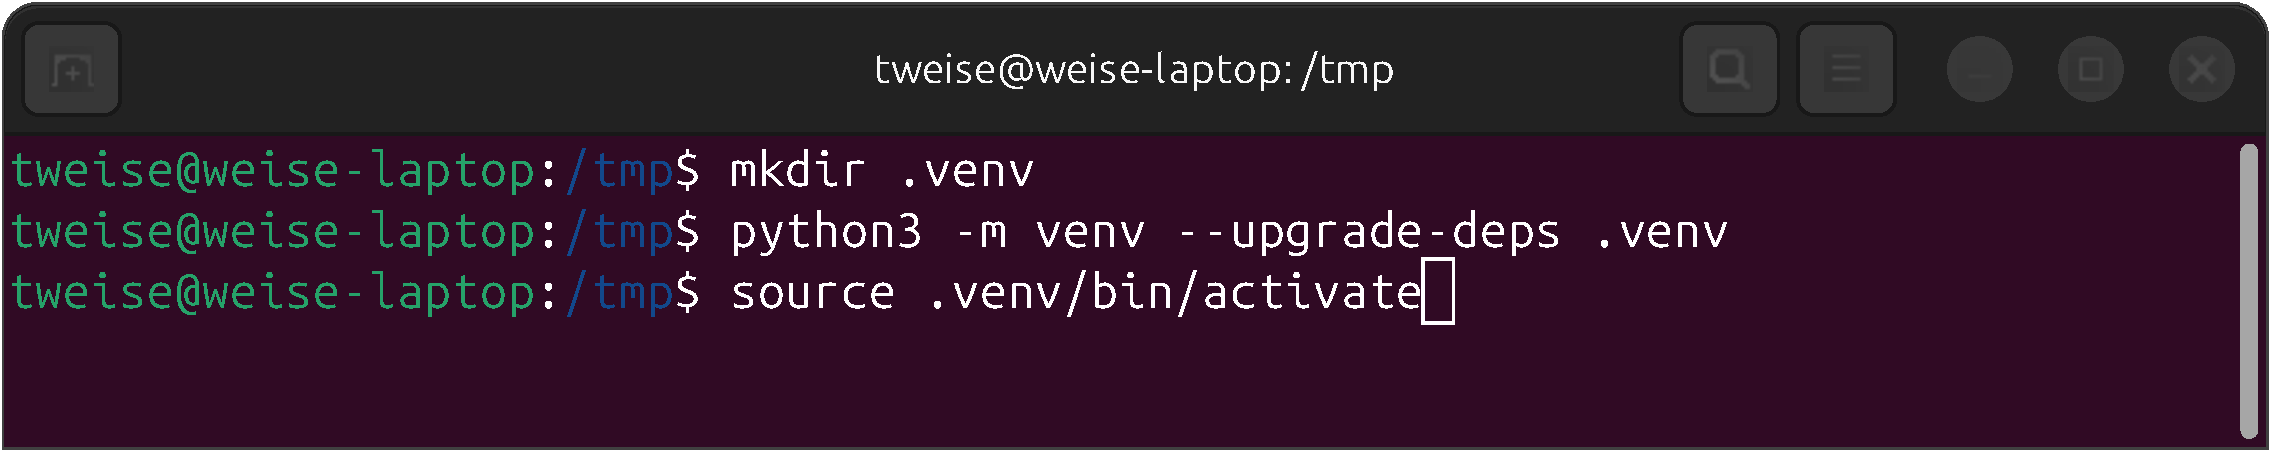
\includegraphics[width=0.7\linewidth]{\currentDir/pipInstallPyscopgVenv3activate}}%
%
\floatRowSep%
%
\subfloat[][%
The \pgls{virtualEnvironment} \textil{.venv} is now active, which we can see by the changed prompt.%
\label{fig:pipInstallPyscopgVenv4activated}%
]{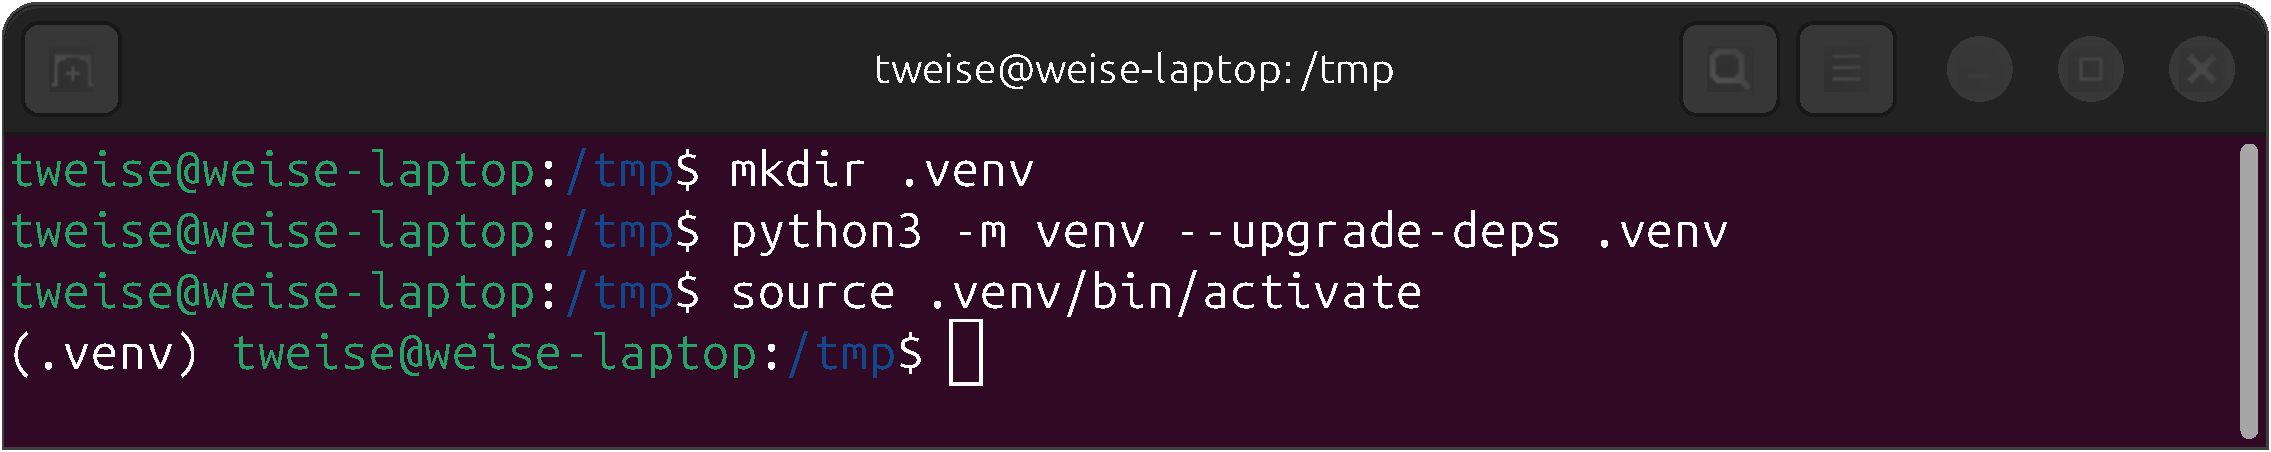
\includegraphics[width=0.7\linewidth]{\currentDir/pipInstallPyscopgVenv4activated}}%
%
\floatRowSep%
%
\subfloat[][%
We install \psycopg\ into this environment by writing \bashil{pip install psycopg} and hitting~\keys{\enter}.%
\label{fig:pipInstallPyscopgVenv5pip}%
]{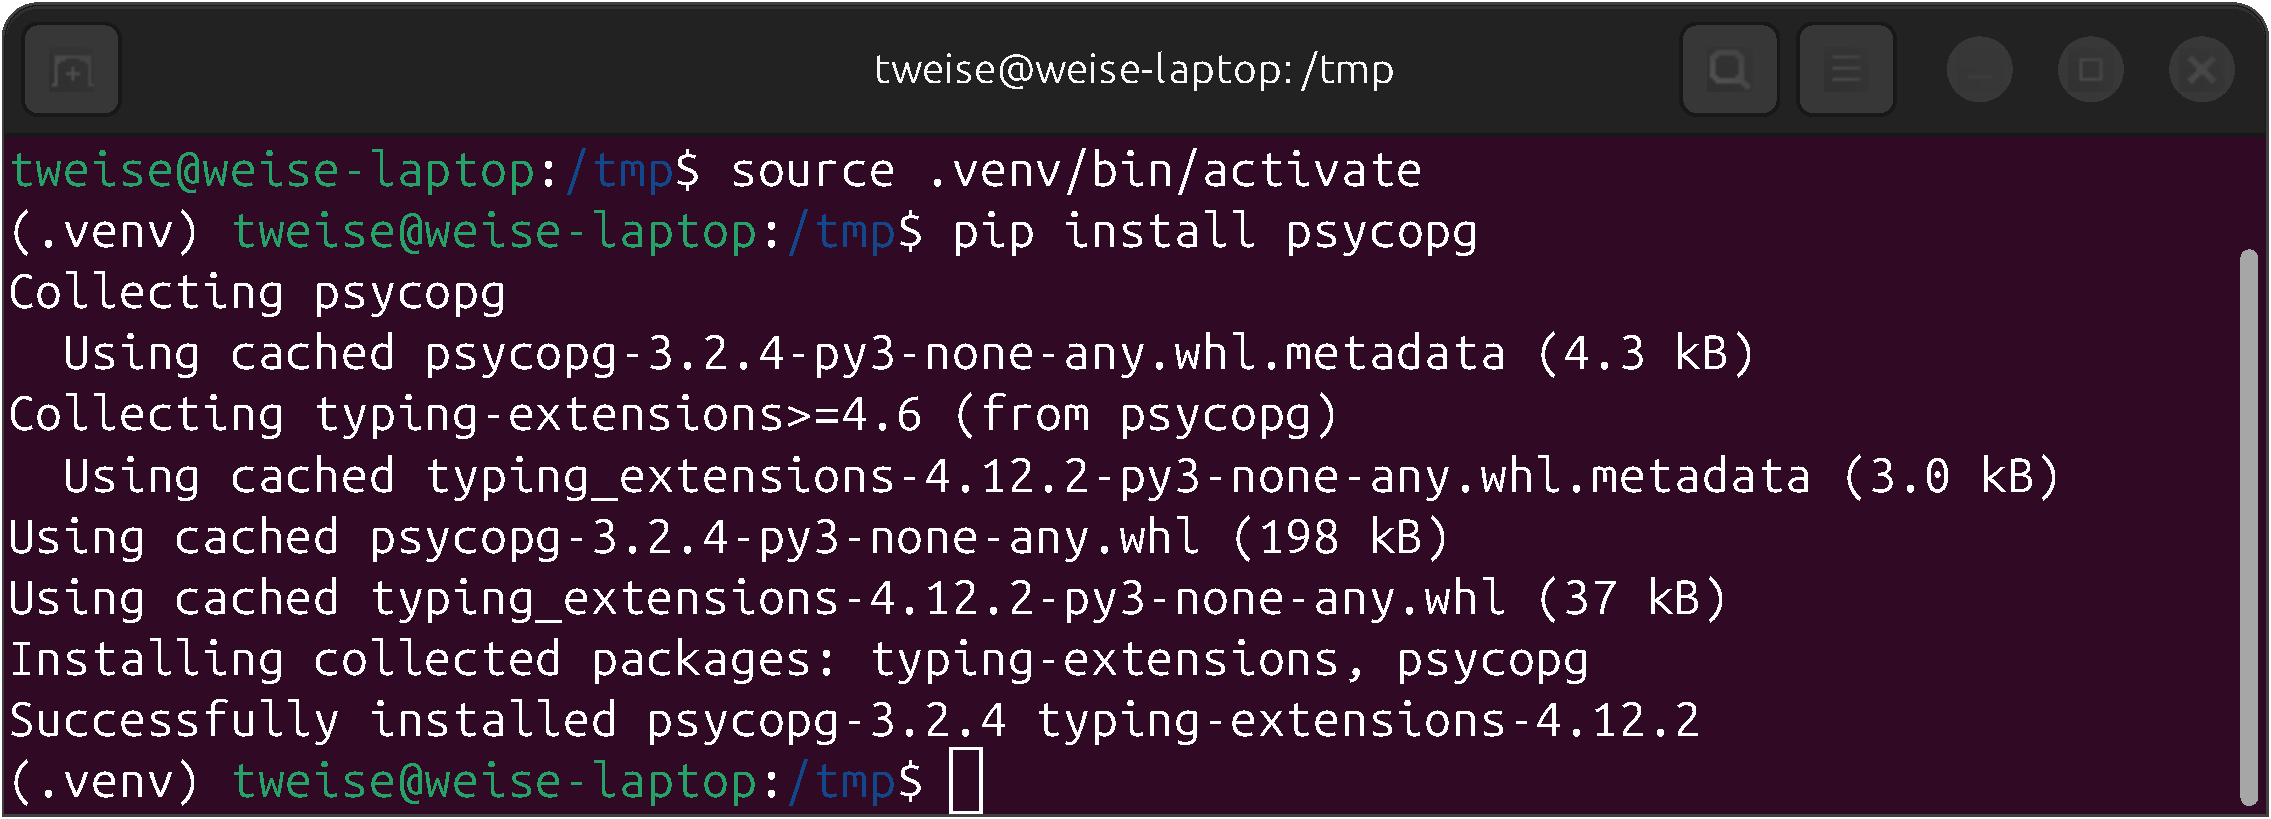
\includegraphics[width=0.7\linewidth]{\currentDir/pipInstallPyscopgVenv5pip}}%
%
\floatRowSep%
%
\subfloat[][%
Once we have finished programming, we can deactivate the \pgls{virtualEnvironment} by writing~\bashil{deactivate} and hitting~\keys{\enter}. %
The prompt changes back to normal.%
\label{fig:pipInstallPyscopgVenv6deactivate}%
]{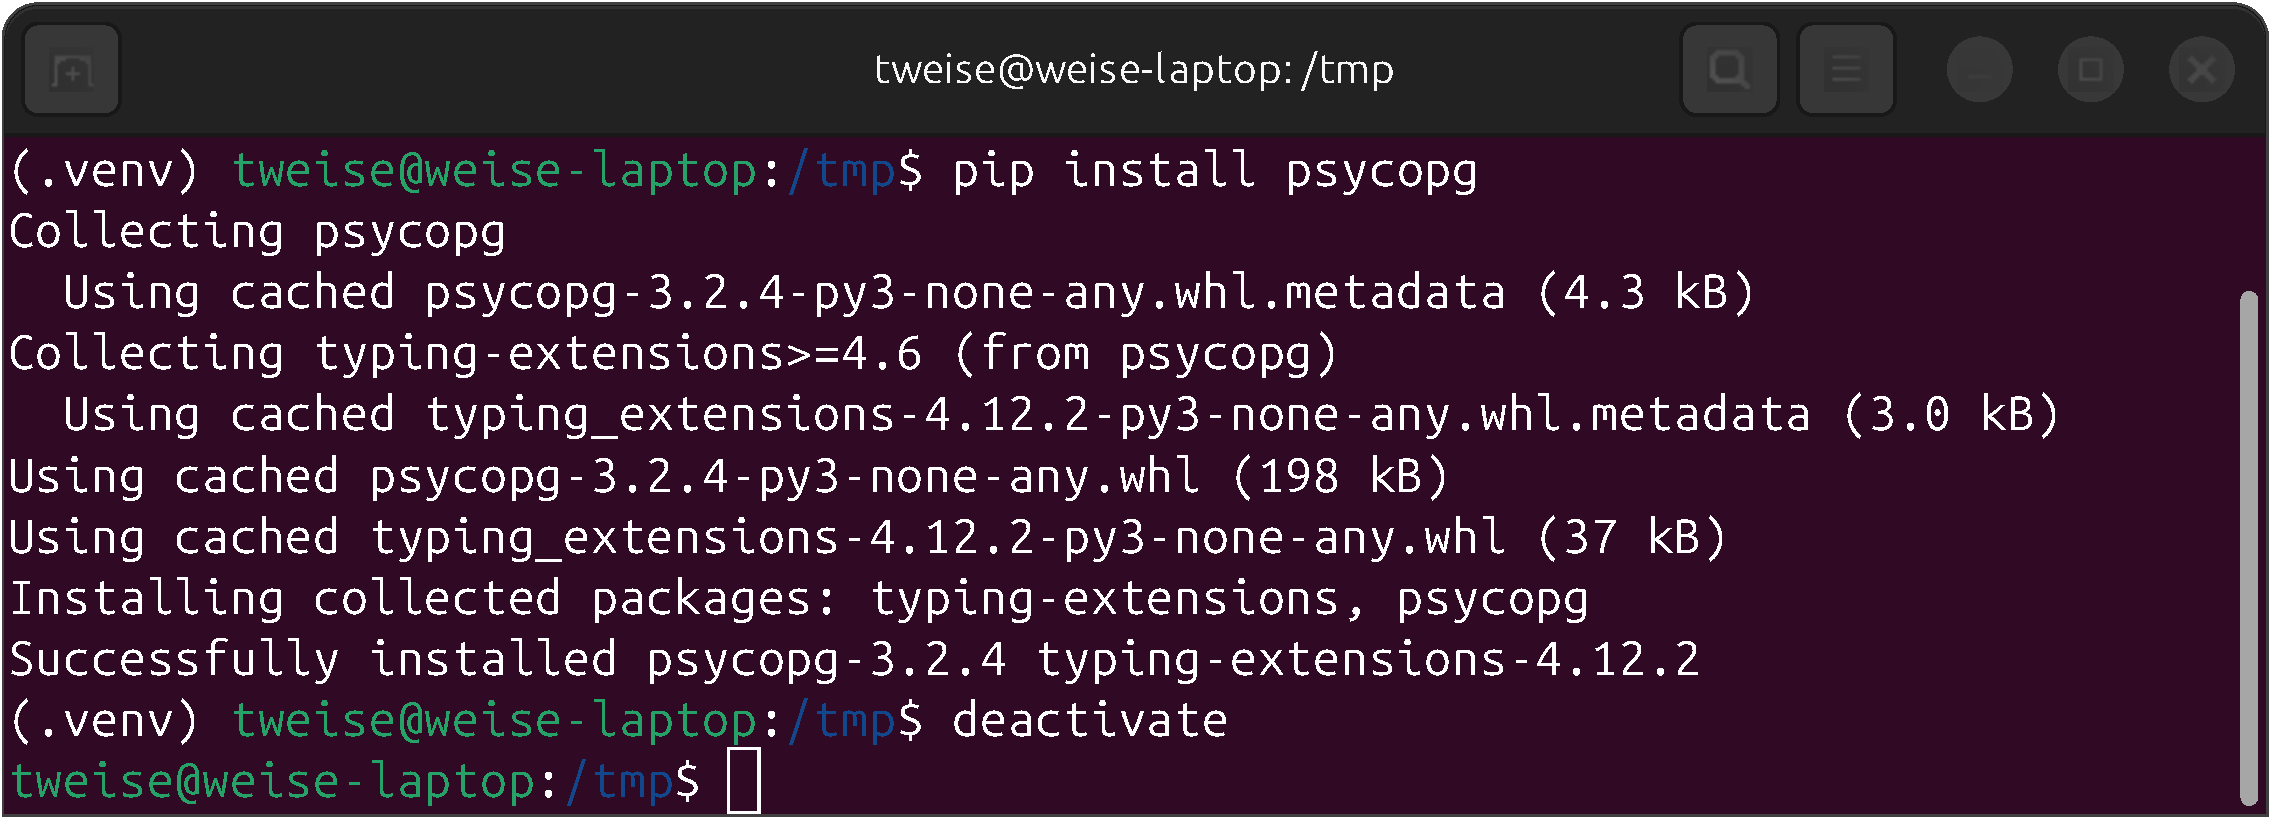
\includegraphics[width=0.7\linewidth]{\currentDir/pipInstallPyscopgVenv6deactivate}}%
%
\caption{Installing the \python\ package \psycopg\ into a \pgls{virtualEnvironment} under \ubuntu\ \linux\ using \pip\ in a \bash\ shell \pgls{terminal}.}%
\label{fig:installPsycopgLinux}%
%
\end{figure}%

The most common way to use external packages in \python\ is to install them into \pglspl{virtualEnvironment}.
A \pgls{virtualEnvironment} is essentially something like a directory hosting a stand-alone \python\ installation separate from the \python\ setup of the computer.
This allows you to have different versions of different libraries installed~(in different \pglspl{virtualEnvironment}).

Imagine that you have one program that requires the \python\ package \numpy\ in version~2.0 or above to run.
You also need to use another application, which can only run with \numpy\ \emph{below} version~2.0.
This is a very common scenario.
It would be impossible to realize, because you can only have one version of \numpy\ installed in your system.
However, you can use both applications if each is installed into its own \pgls{virtualEnvironment}.
Because each \pgls{virtualEnvironment} can have its own version of \numpy.

Therefore, we will first explore this route of installing packages, and we will do so under \ubuntu\ \linux\ in the \bash\ \pgls{terminal} in \cref{fig:installPsycopgLinux}.
For \microsoftWindows, you can find a similar procedure discussed in~\cite{programmingWithPython}.
The commands there are almost the same.

We begin by open a \bash\ \pgls{terminal} using \ubuntuTerminal.
Then we navigate to the directory where our programming will take place.
In my example, I chose the temporary directory \bashil{/tmp} because I will delete everything once I am done taking screenshots.
You would choose a more sensible location.
Inside this directory, we now create a new directory \textil{.venv} to host a new \pgls{virtualEnvironment}.
In the \bash\ shell, we can do this by typing the command \bashil{mkdir .venv} and hitting~\keys{\enter} in \cref{fig:pipInstallPyscopgVenv1mkdir}

After this empty new directory is created, we can instruct \python\ to prepare it for use as a \pgls{virtualEnvironment} in \cref{fig:pipInstallPyscopgVenv2venv}.
We set up a new and empty \pgls{virtualEnvironment} in this directory by writing \bashil{python3 -m venv --upgrade-deps .venv} and hitting~\keys{\enter}.
The new \pgls{virtualEnvironment} has been created.
We now activate it by writing \bashil{source .venv/bin/activate} and hitting~\keys{\enter} in \cref{fig:pipInstallPyscopgVenv3activate}.
Once a \pgls{virtualEnvironment} is active, all package installations will go into that environment.
Also, if we run a \python\ program, it will search for installed packages in this environment.
And our \pgls{virtualEnvironment} \textil{.venv} is now active, which we can see by the changed prompt in \cref{fig:pipInstallPyscopgVenv4activated}.
Notice that the environment is only active in the current \pgls{terminal}.
If you open another \pgls{terminal} using \ubuntuTerminal, our \pgls{virtualEnvironment} is not active in it~(but we can activate it exactly as shown in \cref{fig:pipInstallPyscopgVenv3activate}).

We install \psycopg\ into this environment by writing \bashil{pip install psycopg} and hitting~\keys{\enter}.
This invokes the \pip\ installer, which looks the package up in \pypi\ and downloads it.
In \cref{fig:pipInstallPyscopgVenv5pip}, you see that it downloads \psycopg\ in version~\textil{3.2.4}.
When you do the same thing, you will probably get a newer version installed.

If we run a \python\ program that uses \psycopg, like \cref{lst:factory:connect_insert_and_select}, it will find this version of the package in our \pgls{virtualEnvironment}.
Once we have finished programming and running programs, we can deactivate the \pgls{virtualEnvironment} by writing~\bashil{deactivate} and hitting~\keys{\enter}.
The prompt changes back to normal in \cref{fig:pipInstallPyscopgVenv6deactivate}.
Whenever we need \psycopg\ again, we would activate the \pgls{virtualEnvironment} again as shown in \cref{fig:pipInstallPyscopgVenv3activate}.
Of course, we can also install more packages into this environment.
And we can also create more environments if we want to, in the same way as discussed here.%
\FloatBarrier%
\endhsection%
%
\hsection{Cloning Repository and Installing Psycopg under PyCharm}%
\label{sec:cloningExamplesRepoAndInstallingPsycopgUnderPyCharm}%
%
\begin{figure}%
\centering%
\subfloat[][%
To clone = download the \git\ repository with the examples for this class in the welcome screen of \pycharm, you need to click~\menu{Clone Repository}.%
\label{fig:cloneAndSetupPsycopg01AwelcomeScreenClone}%
]{\tightbox{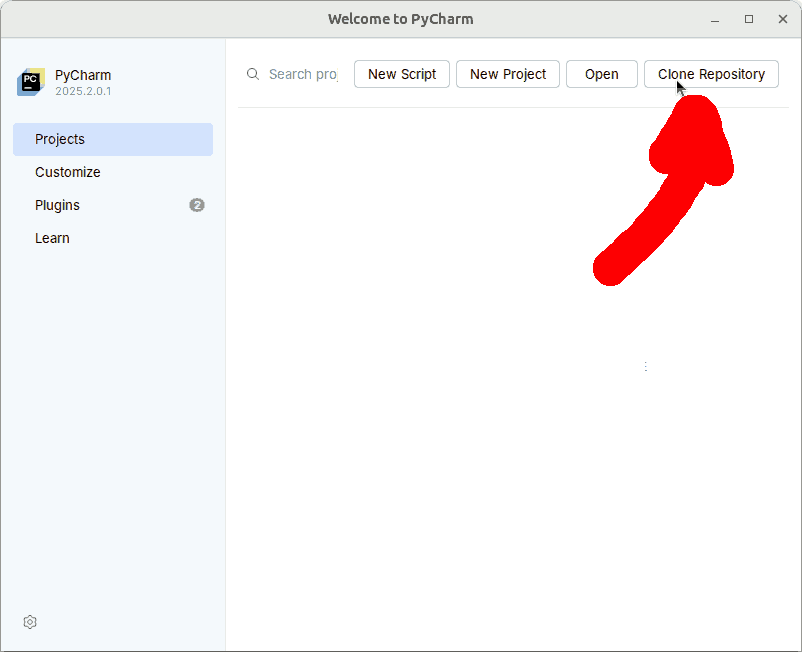
\includegraphics[width=0.45\linewidth]{\currentDir/cloneAndSetupPsycopg01AwelcomeScreenClone}}}%
%
\floatSep%
%
\subfloat[][%
If you are not in the \pycharm\ welcome screen, you can instead click on the \menu{File} menu and then on \menu{Project from Version Control\dots}.%
\label{fig:cloneAndSetupPsycopg01BcloneRepository}%
]{\tightbox{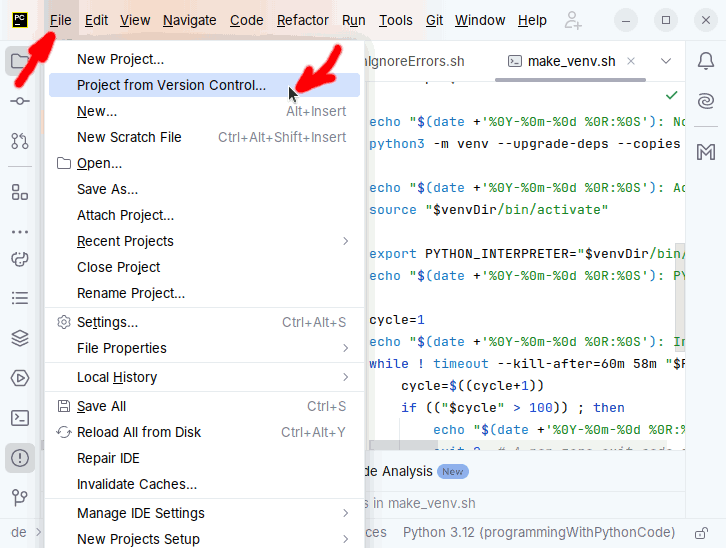
\includegraphics[width=0.45\linewidth]{\currentDir/cloneAndSetupPsycopg01BcloneRepository}}}%
%
\floatRowSep%
%
\subfloat[][%
A new form pops up. %
We have to enter the \git\ repository \pgls{URL} and a location in our local file system to which the repository should be downloaded and where the new \pycharm\ project with its contents should be created.%
\label{fig:cloneAndSetupPsycopg02enterUrl}%
]{\tightbox{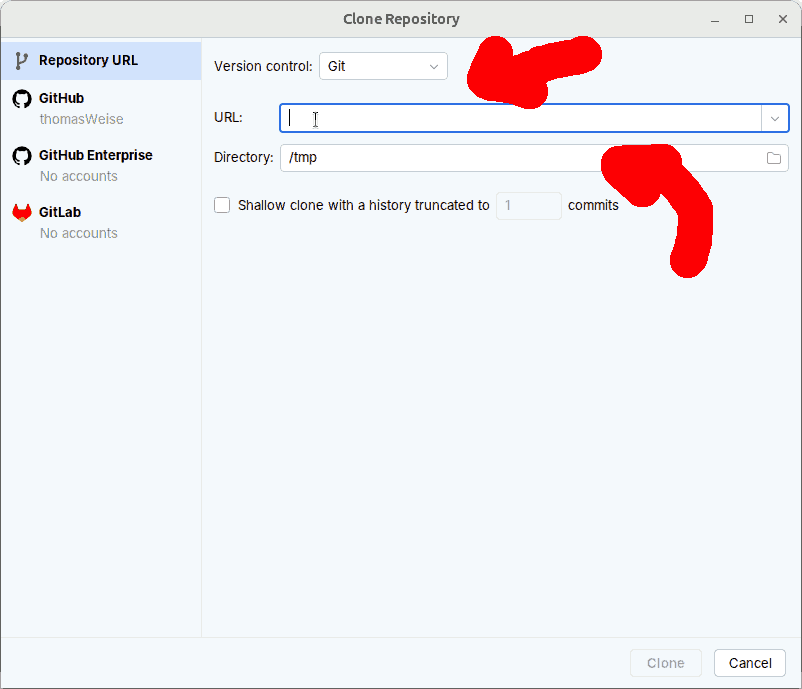
\includegraphics[width=0.45\linewidth]{\currentDir/cloneAndSetupPsycopg02enterUrl}}}%
%
\floatSep%
%
\subfloat[][%
The \pgls{URL} of our repository is \expandafter\url{\databasesCodeRepo}. %
As location, I chose some place in the temporary folder -- you will choose some other place. %
We click on~\menu{Clone}.%
\label{fig:cloneAndSetupPsycopg03urlEntered}%
]{\tightbox{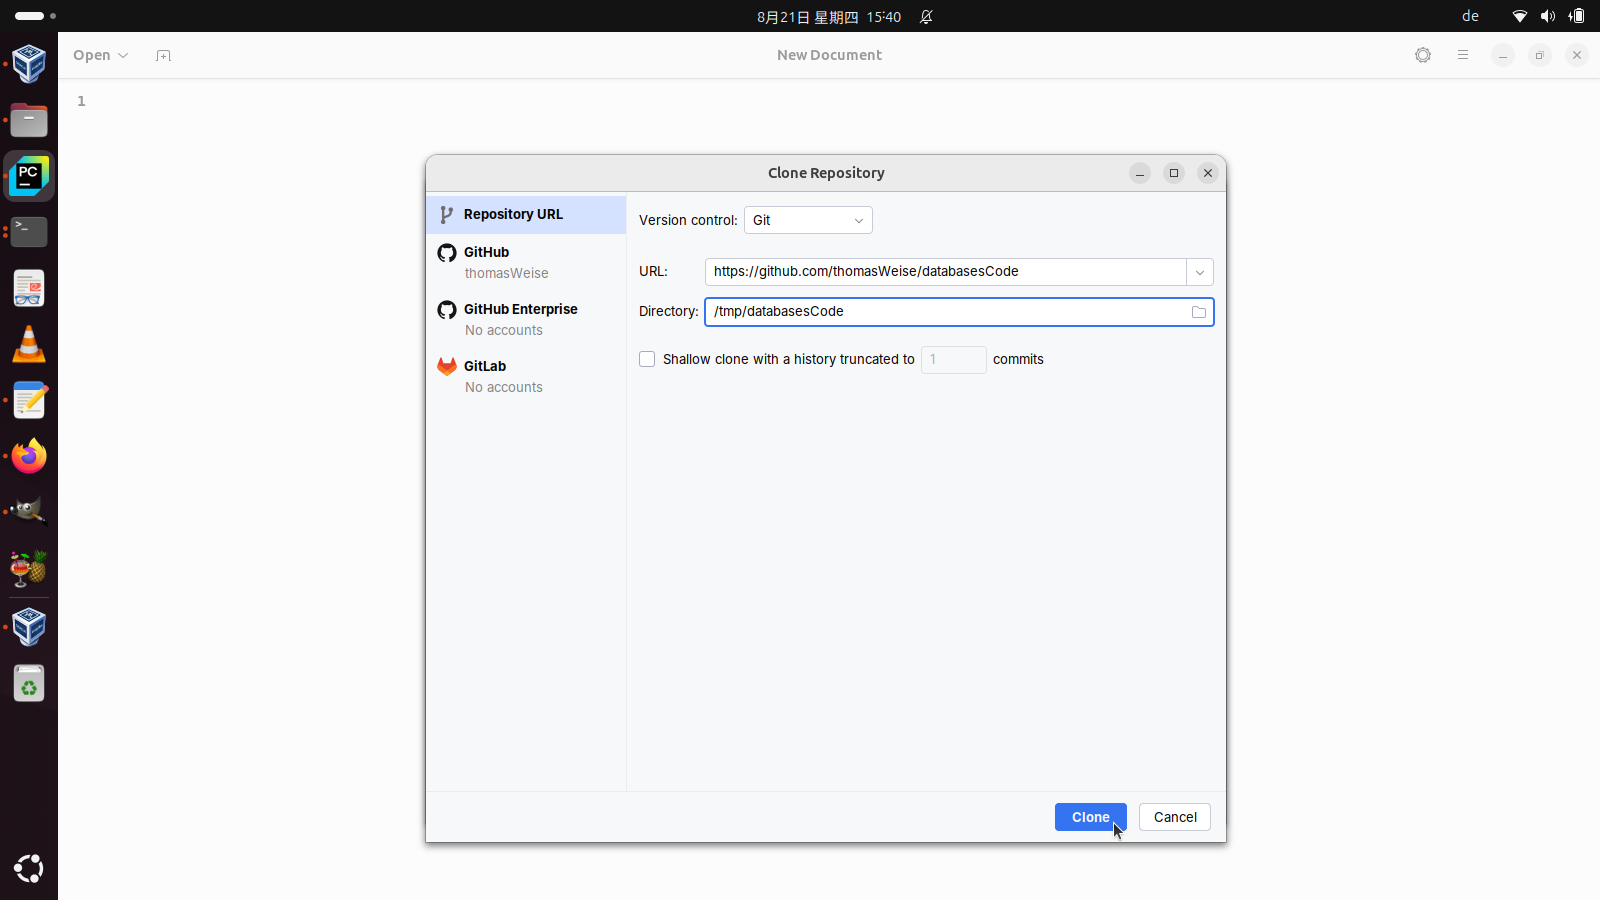
\includegraphics[width=0.45\linewidth]{\currentDir/cloneAndSetupPsycopg03urlEntered}}}%
%
\floatRowSep%
%
\subfloat[][%
The cloning process starts: The repository is downloaded.%
\label{fig:cloneAndSetupPsycopg04cloning}%
]{\tightbox{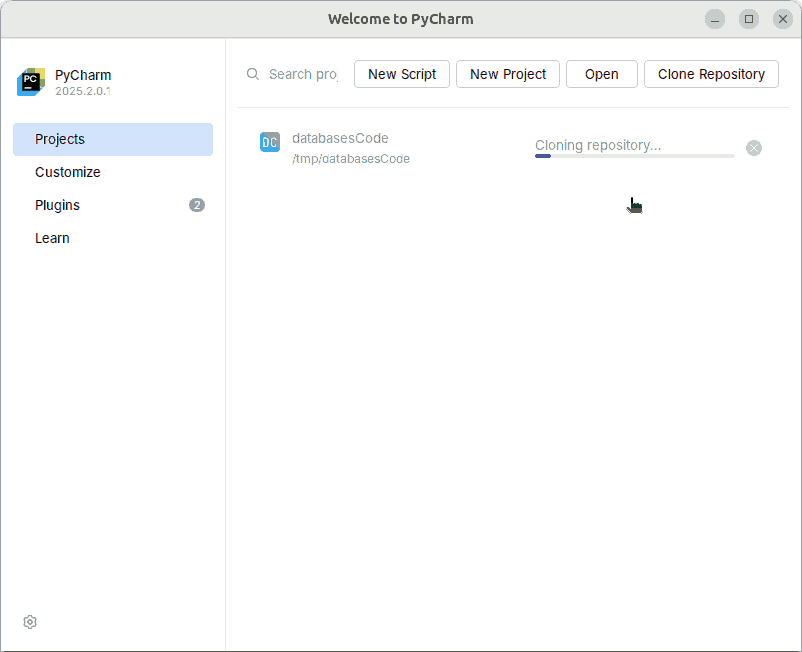
\includegraphics[width=0.45\linewidth]{\currentDir/cloneAndSetupPsycopg04cloning}}}%
%
\floatSep%
%
\subfloat[][%
We may get asked whether we trust this new project. %
After verifying that you downloaded the correct repository, you can click \menu{Trust Project}.%
\label{fig:cloneAndSetupPsycopg05trustQuestion}%
]{\tightbox{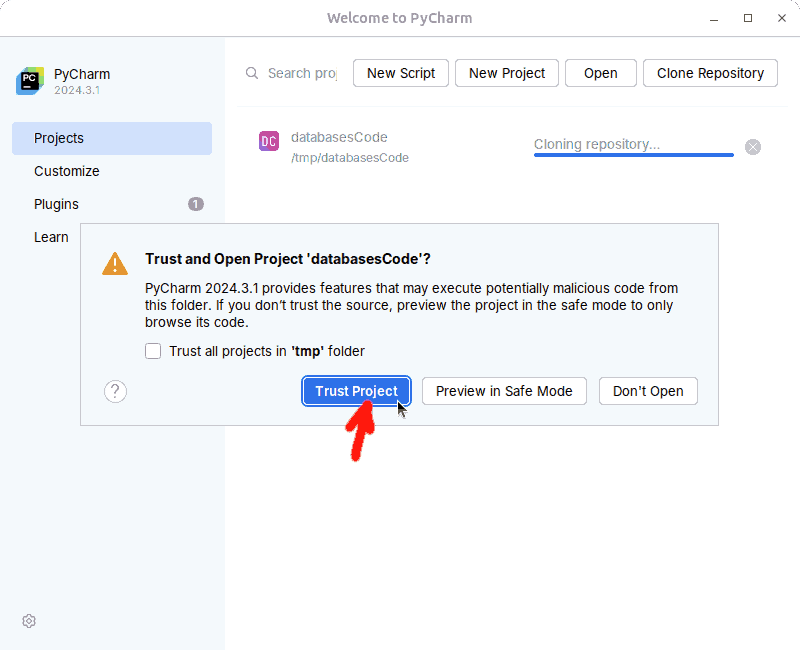
\includegraphics[width=0.45\linewidth]{\currentDir/cloneAndSetupPsycopg05trustQuestion}}}%
%
\caption{Cloning the repository with the examples in \pycharm\ and setting up a \pgls{virtualEnvironment} inside \pycharm\ into which we install \psycopg.}%
\label{fig:cloneAndSetupPsycopgA}%
\end{figure}%
%
\begin{figure}%
\centering%
%
\subfloat[][%
The cloning process is finished. %
The repository has been downloaded. %
Maybe \pycharm\ detects that this project could use \python\ and asks you to configure a \python\ interpreter. %
If you miss this request, see~\cref{fig:cloneAndSetupPsycopg07settings}.%
\label{fig:cloneAndSetupPsycopg06cloned}%
]{\tightbox{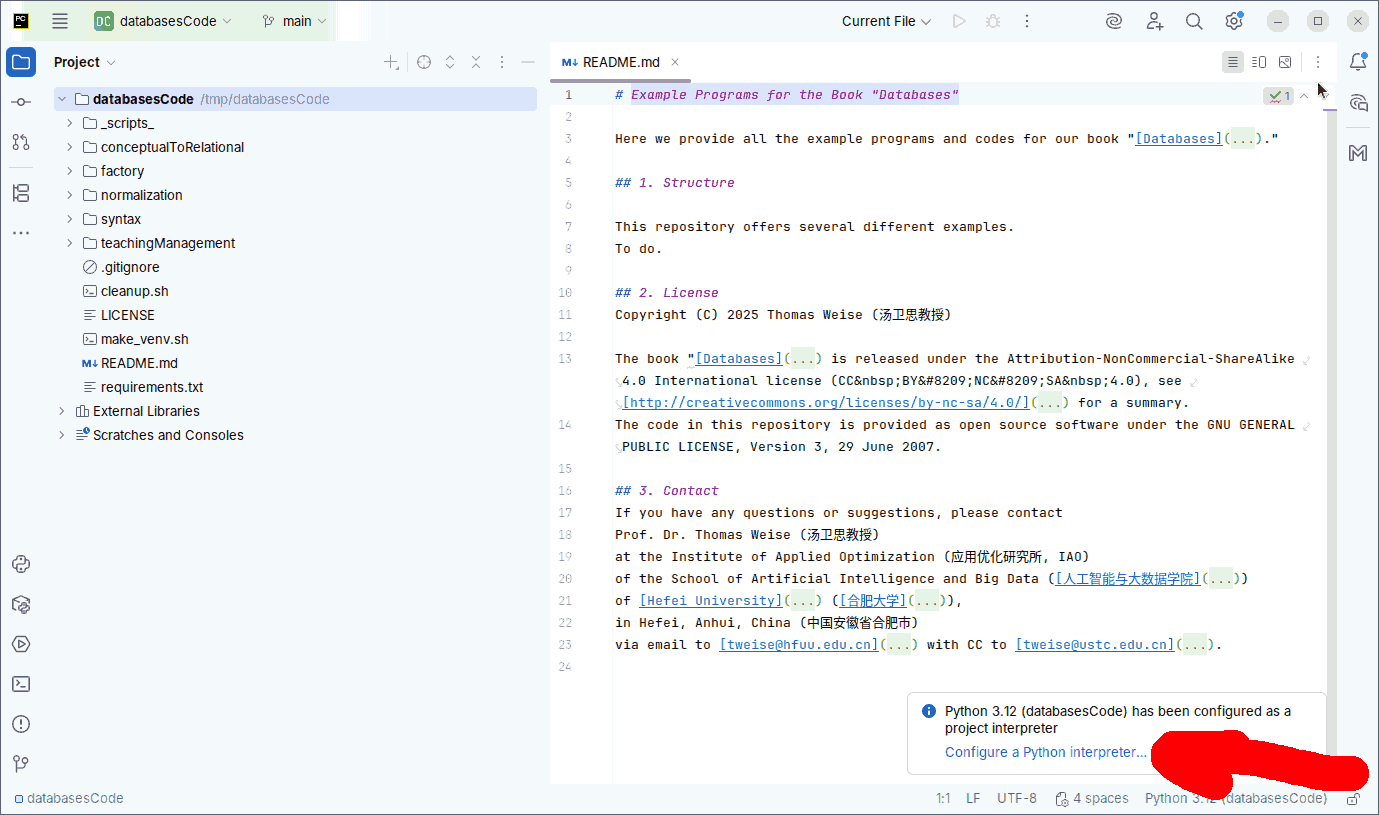
\includegraphics[width=0.45\linewidth]{\currentDir/cloneAndSetupPsycopg06cloned}}}%
%
\floatSep%
%
\subfloat[][%
We now click on the \menu{File} menu and then on~\menu{Settings\dots}, or press \keys{\ctrl+\Alt+S}.%
\label{fig:cloneAndSetupPsycopg07settings}%
]{\tightbox{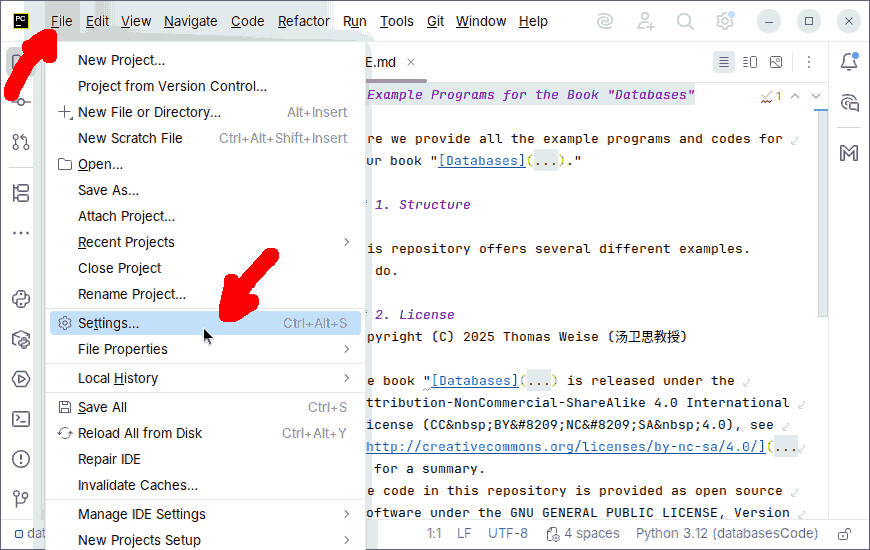
\includegraphics[width=0.45\linewidth]{\currentDir/cloneAndSetupPsycopg07settings}}}%
%
\floatRowSep%
%
\subfloat[][%
We then go to the \menu{Python} settings and choose \menu{Interpreter}. %
There, we click~\menu{Add Interpreter}.%
\label{fig:cloneAndSetupPsycopg08interpreter}%
]{\tightbox{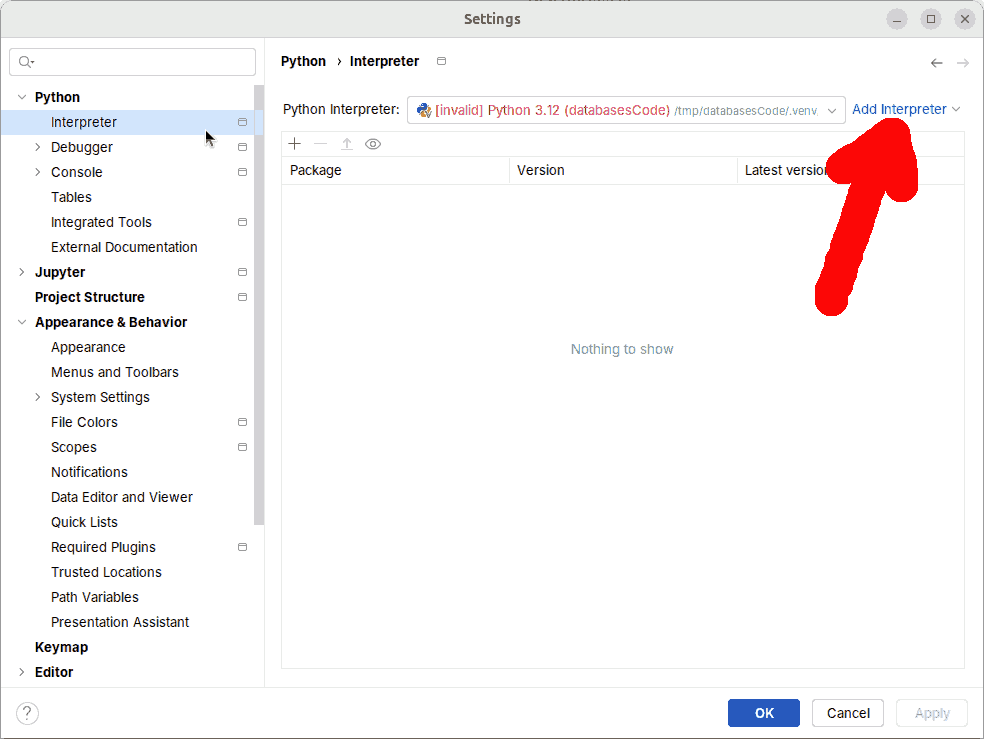
\includegraphics[width=0.45\linewidth]{\currentDir/cloneAndSetupPsycopg08interpreter}}}%
%
\floatSep%
%
\subfloat[][%
{\dots}and then \menu{Add Local Interpreter\dots}.%
\label{fig:cloneAndSetupPsycopg09addLocalInterpreter}%
]{\tightbox{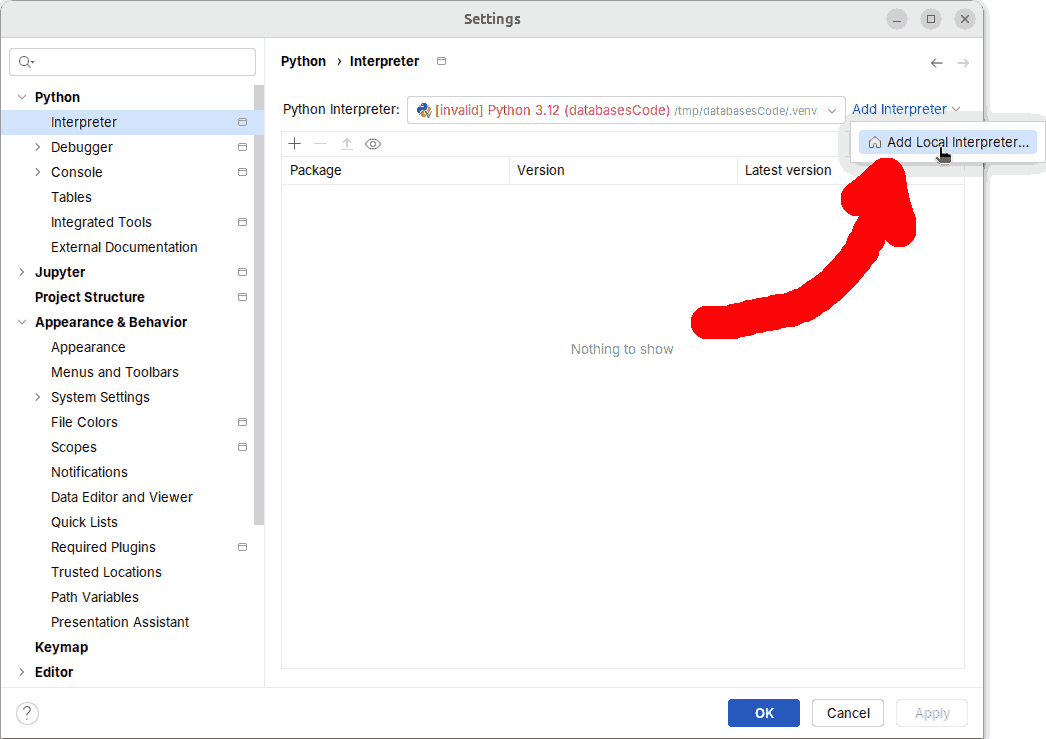
\includegraphics[width=0.45\linewidth]{\currentDir/cloneAndSetupPsycopg09addLocalInterpreter}}}%
%
\floatRowSep%
%
\subfloat[][%
In the dialog that pops open, choose \menu{Generate new}, as type we choose \menu{Virtualenv}, and then we simply add \textil{.venv} as location to the root folder of the project. %
Then we click~\menu{OK}.%
\label{fig:cloneAndSetupPsycopg10localInterpreter}%
]{\tightbox{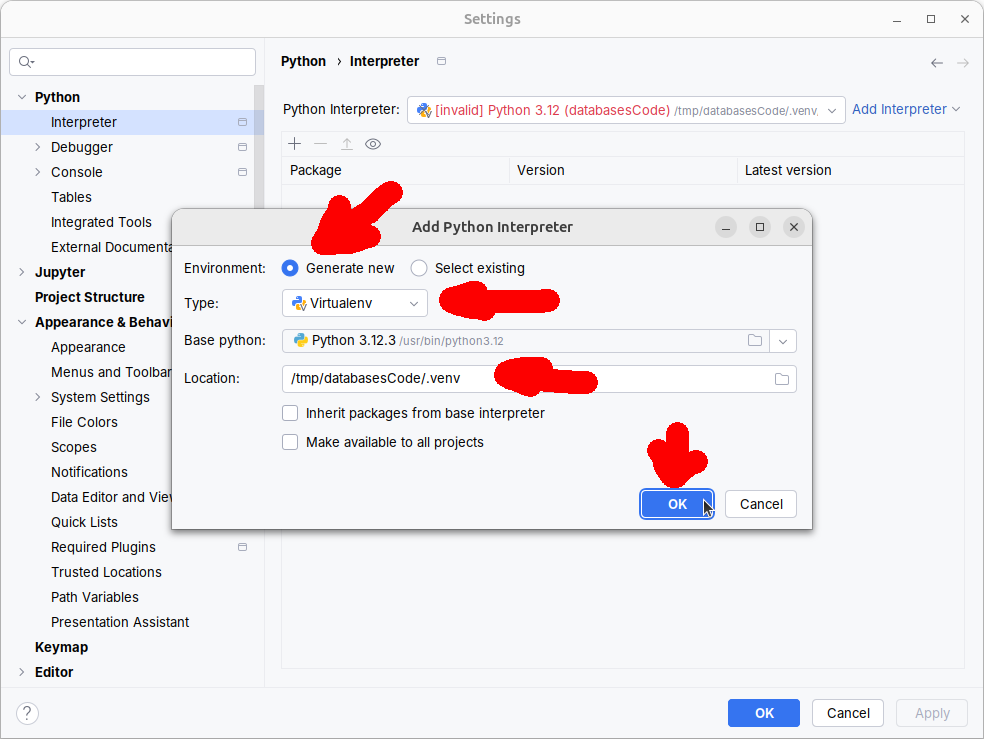
\includegraphics[width=0.45\linewidth]{\currentDir/cloneAndSetupPsycopg10localInterpreter}}}%
%
\floatSep%
%
\subfloat[][%
We click~\menu{OK} again.%%
\label{fig:cloneAndSetupPsycopg11ok}%
]{\tightbox{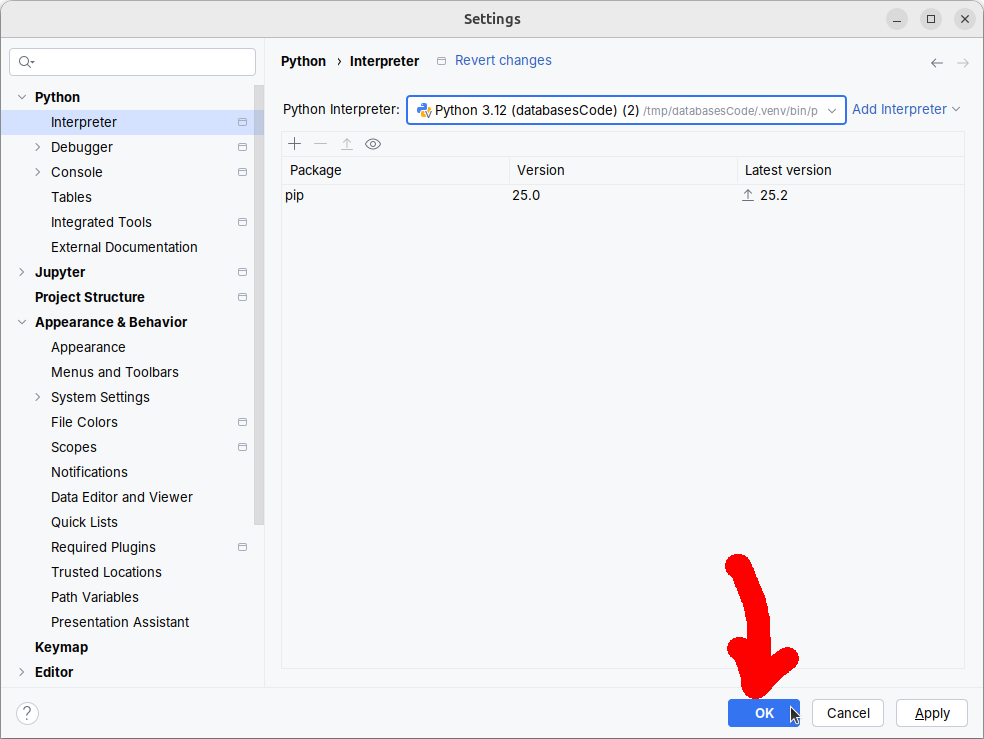
\includegraphics[width=0.45\linewidth]{\currentDir/cloneAndSetupPsycopg11ok}}}%
%
\caption{Cloning the repository with the examples in \pycharm\ and setting up a \pgls{virtualEnvironment} inside \pycharm\ into which we install \psycopg~(Continued).}%
\label{fig:cloneAndSetupPsycopgB}%
\end{figure}%
%
\begin{figure}%
\centering%
%
\subfloat[][%
As you can see, a directory named \textil{.venv} has indeed been created. %
It will host all the files and packages of the environment, which resemble a local \python\ installation.%%
\label{fig:cloneAndSetupPsycopg12venv}%
]{\tightbox{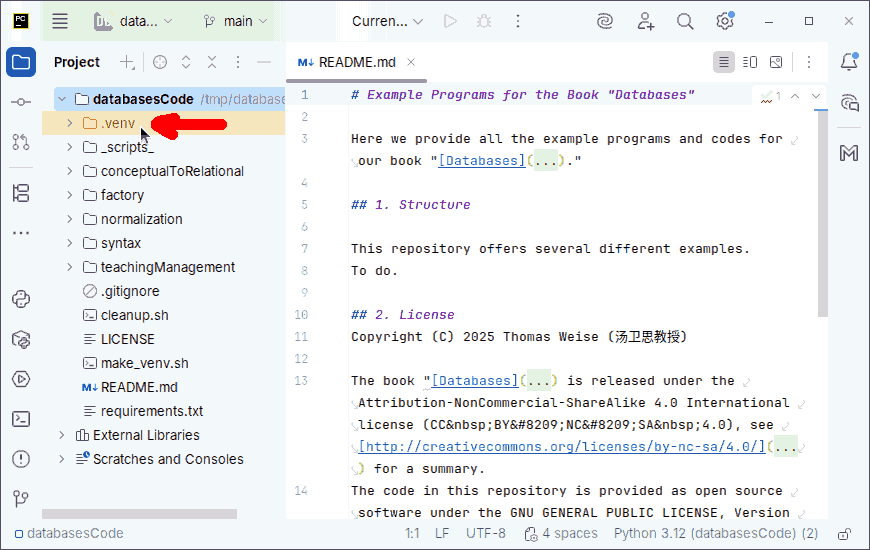
\includegraphics[width=0.45\linewidth]{\currentDir/cloneAndSetupPsycopg12venv}}}%
%
\floatSep%
%
\subfloat[][%
We now click on the file \textil{requirements.txt} in the root folder of the project. %
It lists all the packages required. %
In this case, we need \textil{psycopg} at version~\textil{3.2.4}, which will change in the future.%
\label{fig:cloneAndSetupPsycopg13requirementsTxt}%
]{\tightbox{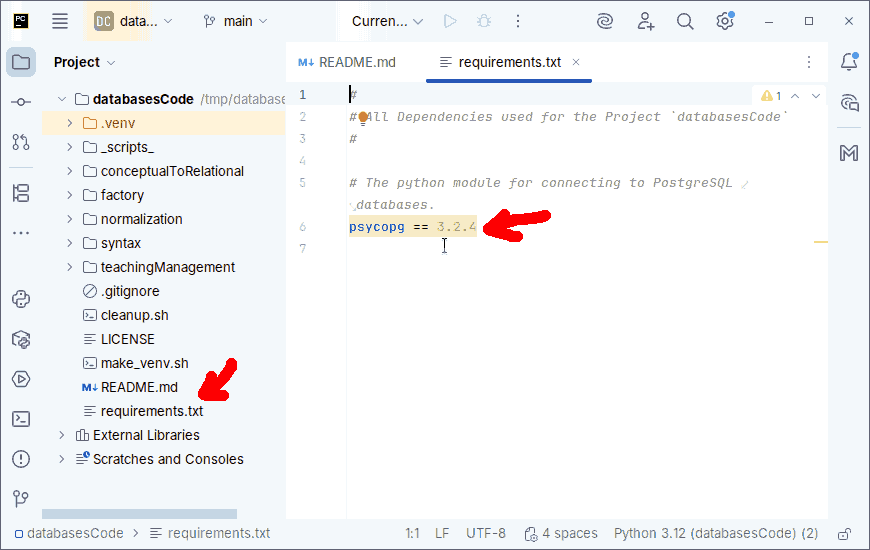
\includegraphics[width=0.45\linewidth]{\currentDir/cloneAndSetupPsycopg13requirementsTxt}}}%
%
\floatRowSep%
%
\subfloat[][%
We right-click on the yellow light bulb symbol, which opens a dialog asking us whether we want to install \psycopg. %
We click on that.%
\label{fig:cloneAndSetupPsycopg14installPackage}%
]{\tightbox{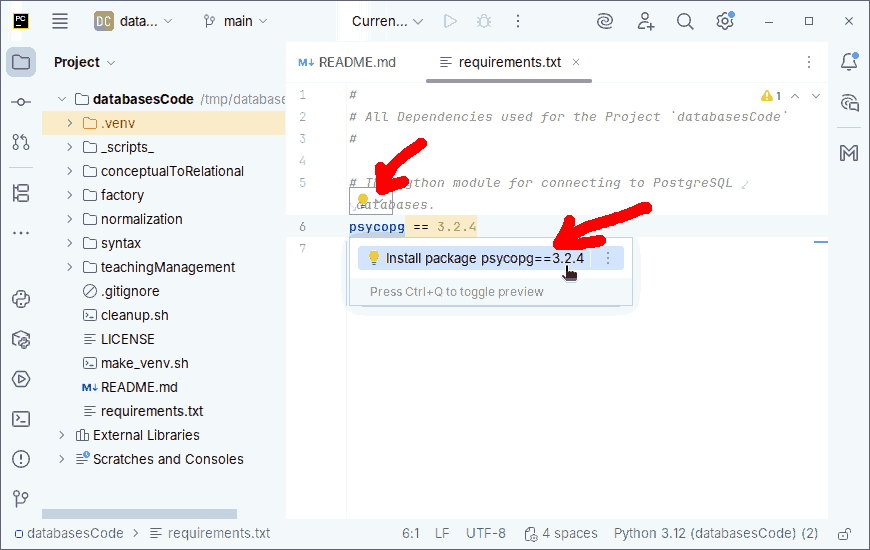
\includegraphics[width=0.45\linewidth]{\currentDir/cloneAndSetupPsycopg14installPackage}}}%
%
\floatSep%
%
\subfloat[][%
We get asked to confirm the package installation. %
We click on~\menu{Yes}.%
\label{fig:cloneAndSetupPsycopg15installPackageOk}%
]{\tightbox{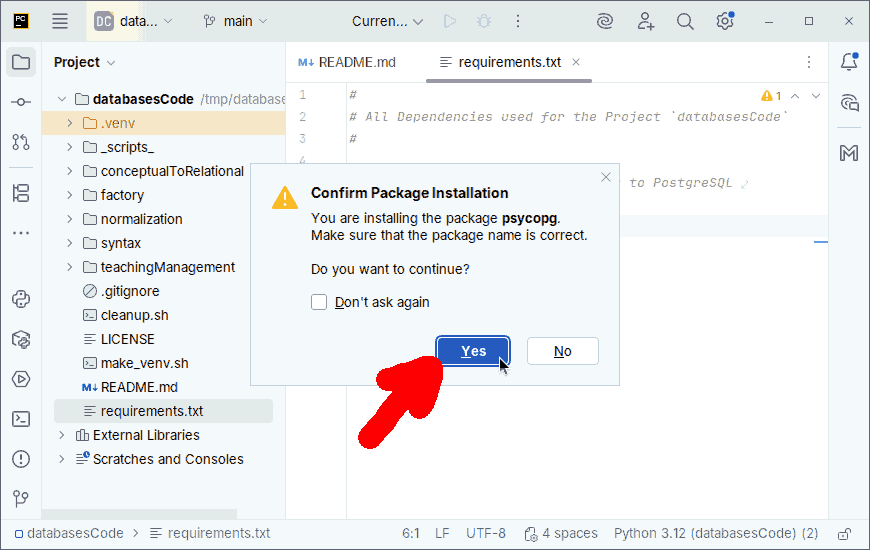
\includegraphics[width=0.45\linewidth]{\currentDir/cloneAndSetupPsycopg15installPackageOk}}}%
%
\floatRowSep%
%
\subfloat[][%
The package is downloaded.%
\label{fig:cloneAndSetupPsycopg16installingPackage}%
]{\tightbox{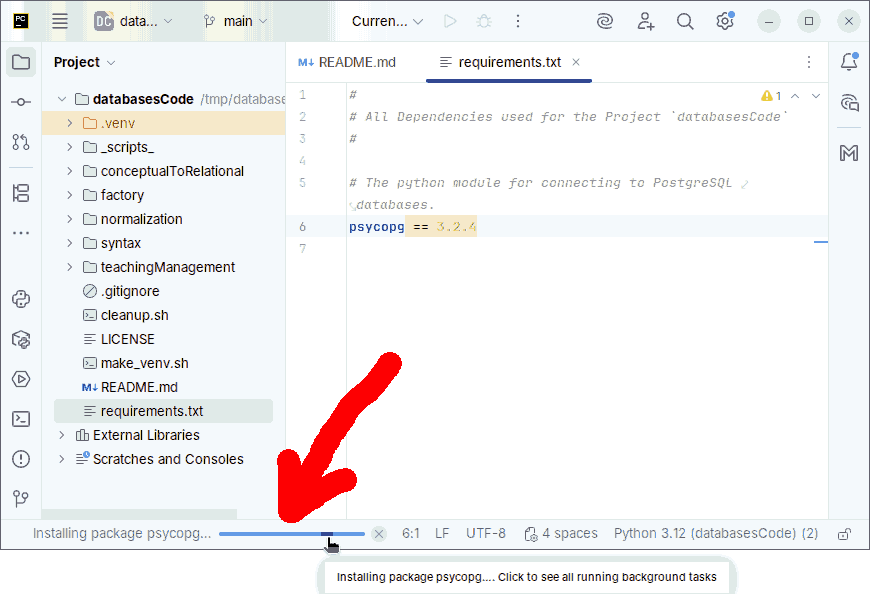
\includegraphics[width=0.45\linewidth]{\currentDir/cloneAndSetupPsycopg16installingPackage}}}%
%
\floatSep%
%
\subfloat[][%
The package is installed. %
Maybe \pycharm\ informs us that a newer version is available.%
\label{fig:cloneAndSetupPsycopg17installedPackage}%
]{\tightbox{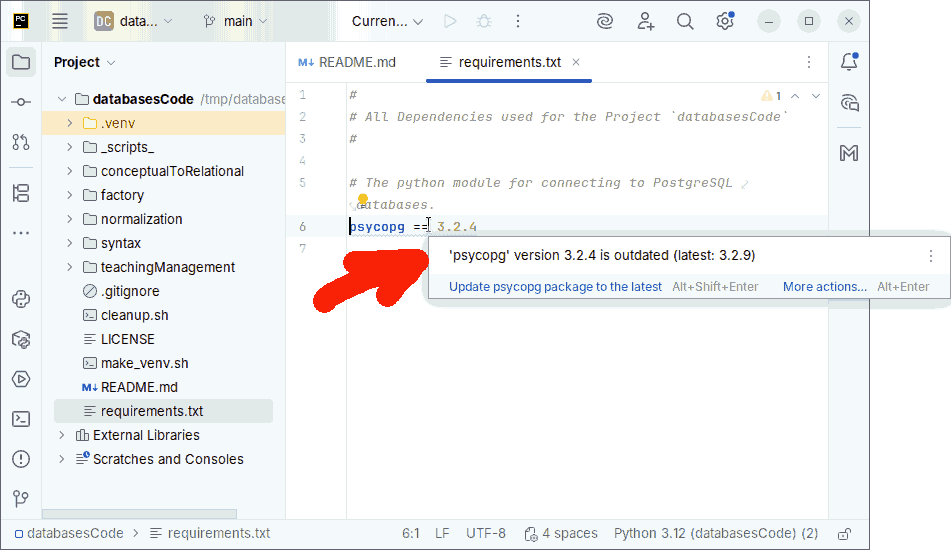
\includegraphics[width=0.45\linewidth]{\currentDir/cloneAndSetupPsycopg17installedPackage}}}%
%
%
\caption{Cloning the repository with the examples in \pycharm\ and setting up a \pgls{virtualEnvironment} inside \pycharm\ into which we install \psycopg~(Continued).}%
\label{fig:cloneAndSetupPsycopgC}%
\end{figure}%
%
\begin{figure}%
\centering%
%
\subfloat[][%
Indeed, we can now even find it in the \textil{.venv} folder.%%
\label{fig:cloneAndSetupPsycopg18installedPackageInVenv}%
]{\tightbox{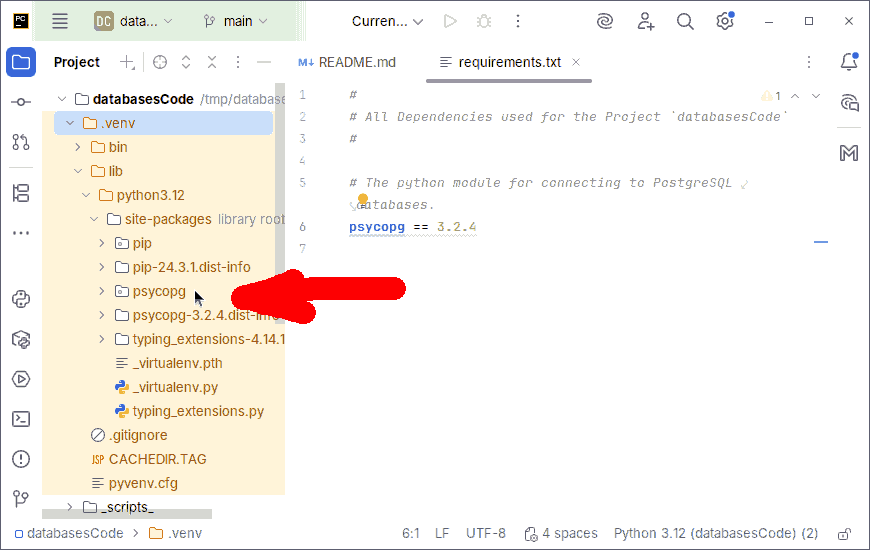
\includegraphics[width=0.8\linewidth]{\currentDir/cloneAndSetupPsycopg18installedPackageInVenv}}}%
%
%
\caption{Cloning the repository with the examples in \pycharm\ and setting up a \pgls{virtualEnvironment} inside \pycharm\ into which we install \psycopg~(Continued).}%
\label{fig:cloneAndSetupPsycopgD}%
\end{figure}%
%
\git\ is a distributed \pgls{VCS}, meaning that it allows us to create so-called repositories, which basically are directories, whose change history is preserved and that can be collaboratively edited by teams.
Every team member has a local copy of the code and can commit their local changes to the central repository as well as download the changes comitted by others.
\github\ is one provider that offers us to host \git\ repositories online.
All the example files used in this book are stored in such a \git\ repository on \github:~\expandafter\url{\databasesCodeRepo}.

The process of downloading a \git\ repository with all its history is called \emph{cloning}.
\pycharm\ is an \pgls{ide} for \python\ software development that supports \git.
You can use it to clone \git\ repositories and it also supports using local \pglspl{virtualEnvironment} as well as installing packages into them based on the requirements that a repository defines.
Since we want to access \postgresql\ \pglspl{db} from \python\ using \psycopg, our example repository does specify this package as a dependency.

Thus, it is possible to clone our example repository and install \psycopg\ in one step.
This can be done as follows.

First, we need to open \pycharm\ and then clone the repository.
This can be done by clicking the \menu{Clone Repository} button in the \pycharm\ welcome screen, as illustrated in~\cref{fig:cloneAndSetupPsycopg01AwelcomeScreenClone}.
If you don't have that welcome screen open, you can also click on the \menu{File} menu and then on \menu{Project from Version Control\dots}, as shown in~\cref{fig:cloneAndSetupPsycopg01BcloneRepository}.
Then, a new form pops up in~\cref{fig:cloneAndSetupPsycopg02enterUrl}.
We have to enter the \git\ repository \pgls{URL} and a location in our local file system to which the repository should be downloaded and where the new \pycharm\ project with its contents should be created.

As said, the \pgls{URL} of our repository is \expandafter\url{\databasesCodeRepo}.
As location, I chose some place in the temporary folder in~\cref{fig:cloneAndSetupPsycopg03urlEntered}, because I am just making screenshots for this book and will delete the project afterwards.
You will choose some other, more reasonable and permanent place.
We click on \menu{Clone} and the cloning process starts in \cref{fig:cloneAndSetupPsycopg04cloning}.
We may get asked whether we trust this new project.
After verifying that you downloaded the correct repository, you can click \menu{Trust Project}, as shown in~\cref{fig:cloneAndSetupPsycopg05trustQuestion}.

Eventually the cloning process is finished.
The repository has been downloaded.
Maybe \pycharm\ detects that this project could use \python\ and asks you to configure a \python\ interpreter as shown in~\cref{fig:cloneAndSetupPsycopg06cloned}.
In my case, this request disappeared too quickly, so in~\cref{fig:cloneAndSetupPsycopg07settings}, I instead clicked on the \menu{File} menu and then on~\menu{Settings\dots}, or press \keys{\ctrl+\Alt+S}.
Either way, we would go to the \menu{Python} settings and choose \menu{Interpreter}.
There, we click~\menu{Add Interpreter} in \cref{fig:cloneAndSetupPsycopg08interpreter} and then \menu{Add Local Interpreter\dots}~(\cref{fig:cloneAndSetupPsycopg09addLocalInterpreter}).

In the dialog that pops open, we choose \menu{Generate new}.
As type we choose \menu{Virtualenv}.
The \pgls{virtualEnvironment} is basically a directory which contains a local \python\ installation.
This allows us to have separate \python\ setups for different projects.
Therefore, if our course requires you to work with a version of \psycopg\ but your other projects do not need that, then you would only install it into the local \pgls{virtualEnvironment} for the examples of our course.
If \psycopg, in turn, requires other libraries, then these will live in this separate \pgls{virtualEnvironment}, too.
Therefore, nasty things like version conflicts with the setups of other projects cannot occur.
We add \textil{.venv} as location for this \pgls{virtualEnvironment} to the root folder of the project.
Then we click~\menu{OK} in \cref{fig:cloneAndSetupPsycopg10localInterpreter}.
We click~\menu{OK} again in \cref{fig:cloneAndSetupPsycopg11ok}.
As you can see in~\cref{fig:cloneAndSetupPsycopg12venv}, a directory named \textil{.venv} has indeed been created.
It will host all the files and packages of the environment, which resemble a local \python\ installation.

The packages that a \python\ project requires are usually listed in a file called \textil{requirements.txt}.
Such a file is also present in the root folder of our example repository.
We click on it in \pycharm\ and find that it indeed lists all the packages required:
We need \textil{psycopg} at version~\textil{3.2.4} as shown in \cref{fig:cloneAndSetupPsycopg13requirementsTxt}.
Of course, this is only at the time of this writing and will change in the future.

Anyway, when we explore this file, we can see some yellow hints and a yellow light bulb symbol.
We click on it and it opens a dialog asking us whether we want to install \psycopg.
We then click on that in~\cref{fig:cloneAndSetupPsycopg14installPackage}.
\pycharm\ asks us to confirm the package installation, which we do, by clicking on~\menu{Yes} in~\cref{fig:cloneAndSetupPsycopg15installPackageOk}

\pycharm\ now downloads the package for us in~\cref{fig:cloneAndSetupPsycopg16installingPackage} and then installs it into the \pgls{virtualEnvironment}.
Maybe \pycharm\ informs us that a newer version is available, as shown in~\cref{fig:cloneAndSetupPsycopg17installedPackage}.
Anyway, we can see that the package has been included in the \textil{.venv} folder, as illustrated in~\cref{fig:cloneAndSetupPsycopg18installedPackageInVenv}.
It is now available for our experiments.%
%
\FloatBarrier%
\endhsection%
%
\endhsection%
%
